\subsection{Упражнение 1}

Скачайте с сайта http://freesound.org , включающий музыку, речь или иные звуки, имеющие четко выраженную высоту. Выделите примерно полусекундный сегмент, в котором высота постоянна. Вычислите и распечатайте спектр выбранного сегмента. Как связаны тембр звука и гармоническая структура, видимая в спектре?


\noindent Используйте high\_pass, low\_pass, и band\_stop для фильтрации тех или иных гармоник. Затем преобразуйте спектры обратно в сигнал и прослушайте его. Как звук соотносится с изменениями, сделанными в спектре?
    

Загружаем звуки игры на пианино, взятые на сайте freesound.org и загруженные на мой репозиторий. Добавляем звуки в класс Wave. Поделим исходную запись на фрагменты и вырежем одну часть.

\begin{lstlisting}[language=Python]
if not os.path.exists('1647_piano.wav'):
    !wget https://github.com/pimenov01/telecom/raw/
    main/files/1647_piano.wav
wave = read_wave('1647_piano.wav')
wave.make_audio()
wave = wave.segment(18.3,0.5)
wave.make_audio()
read_wave('1647_piano.wav').plot().plot()
wave.plot()
\end{lstlisting}
    
\begin{figure}[H]
	\begin{center}
		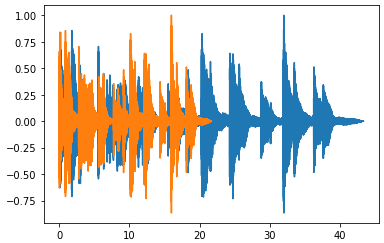
\includegraphics[scale=1]{fig/lab01/lab1_1.png}
		\caption{График фрагмента звука}
	\end{center}
\end{figure}

Далее узнаем спектр звука при помощи метода make\_spectrum и построим график для наглядности.
\begin{lstlisting}[language=Python]
spectrum = wave.make_spectrum()
spectrum.plot(high=5000)
\end{lstlisting}

\begin{figure}[H]
	\begin{center}
		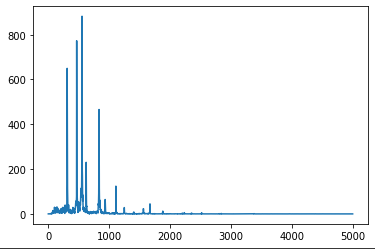
\includegraphics[scale=1]{fig/lab01/lab1_2.png}
		\caption{Спектр звука}
	\end{center}
\end{figure}

Мы видим, что данные расположились до 2Кгц, а график получился не информативный. Обрежем частоты выше 1250Гц, т.к. до них хранится вся важная информация - пики. На остальное смотреть не будем.

\begin{figure}[H]
	\begin{center}
		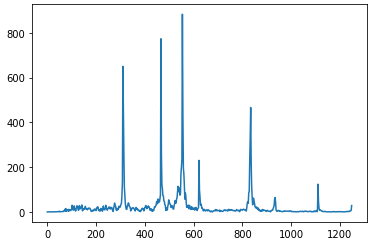
\includegraphics[scale=1]{fig/lab01/lab1_3.png}
		\caption{Спектр звука, частота меньше 1250 ГЦ}
	\end{center}
\end{figure}

Для точного понимания какие ноты сыграны выведем список пиков частот в спектре:

\begin{lstlisting}[language=Python]
spectrum.peaks()[:10]
\end{lstlisting}

\begin{lstlisting}
[(882.3500533686324, 554.0),
 (772.8812508117549, 466.0),
 (649.662314039115, 310.0),
 (466.0353893832775, 834.0),
 (455.88324114785496, 312.0),
 (435.6400663619303, 556.0),
 (328.0318016013845, 832.0),
 (260.99365239113706, 314.0),
 (251.02745102094198, 468.0),
 (234.35739758178494, 552.0)]
\end{lstlisting}


Находим соответствие музыкальных нот и частот из пиков:
\begin{itemize}
\item 554.36 Гц - С\# II
\item 466.16 Гц -  A\# I
\item 311.13 Гц - D\# I
\item 830.60 Гц - G\# II
\end{itemize}
Где \# обозначает "диез" или же черную ноту, римские цифра обозначают октаву ноты. У C\# II самая большая амплитуда, поэтому 554.36 Гц - доминирующая частота. Общая воспринимаемая высота звука зависит от основной частоты, тут она 311.13 Гц.

Добавим фильтр нижних частот. Все компоненты выше 540 ГЦ будут удалены. (На самом деле можно выбирать на сколько их ослаблять, но я решил на 100\%).

\begin{lstlisting}[language=Python]
spectrum2 = wave.make_spectrum()
spectrum2.low_pass(540)
spectrum2.plot(high=1000)
\end{lstlisting}

\begin{figure}[H]
	\begin{center}
		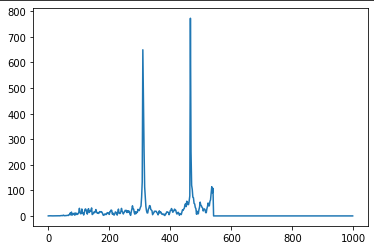
\includegraphics[scale=1]{fig/lab01/lab1_4.png}
		\caption{Спект с фильтром нижних частот}
	\end{center}
\end{figure}

Добавим фильтр верхних частот, и ослабим на половину компоненты до 500 Гц.

\begin{lstlisting}[language=Python]
spectrum2.high_pass(500,0.5)
spectrum2.plot(high=1000)
\end{lstlisting}

\begin{figure}[H]
	\begin{center}
		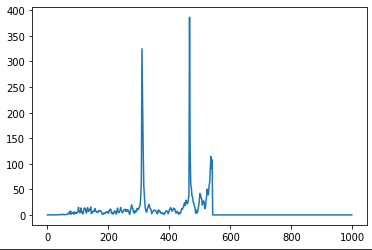
\includegraphics[scale=1]{fig/lab01/lab1_5.png}
		\caption{Спект с фильтром верхних частот}
	\end{center}
\end{figure}

Уберём частоты между Ре и Ля.

\begin{lstlisting}[language=Python]
spectrum2.band_stop(320,450)
spectrum2.plot(high=1000)
\end{lstlisting}



\begin{figure}[H]
	\begin{center}
		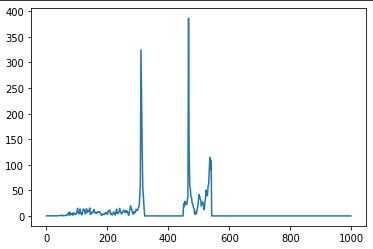
\includegraphics[scale=1]{fig/lab01/lab1_6.png}
		\caption{Получившийся спектр}
	\end{center}
\end{figure}

Звучание заметно изменилось из-за изменения доиминирующей частоты (её ампилитуда была уменьшена в 2 раза), но напоминает изначальный отрезок.

\begin{lstlisting}[language=Python]
wave = read_wave('1647_piano.wav')
wave = wave.segment(18.3,0.5)
spectrum2 = wave.make_spectrum()
spectrum2.high_pass(500)
spectrum2.plot(high=1000)
\end{lstlisting}

\begin{figure}[H]
	\begin{center}
		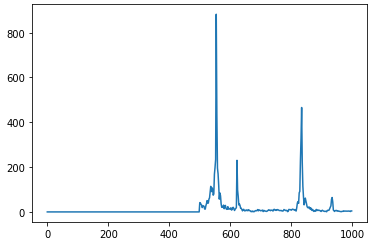
\includegraphics[scale=1]{fig/lab01/lab1_7.png}
		\caption{Отфильтрованные нижние компоненты}
	\end{center}
\end{figure}

Отфильтровав нижние частоты звук стал более высоким. Это логично, ведь ннизкие частоты придают более гулкое звучание, а на получившейся дорожке убраны все частоты, ниже 500.

\subsection{Упражнение 2}

Создайте сложный сигнал из объектов SinSignal и CosSignal, суммируя их. Обработайте сигнал для получения wave и прослушайте его. Вычислите Spectrum и распечатайте. Что произойдёт при добавлении частотных компонент, не кратных основным?


Берём два сигнала с частотой одной октавы. В итоге мы должны получить классическую синусоиду - волновой сигнал с очень высоким звучанием, однако из него при желании можно сделать бас, если опустить на несколько октав ниже.
\begin{lstlisting}[language=Python]
from thinkdsp import SinSignal, CosSignal
# https://nch-nch.ru/apps/frequency/
cos_sig1 = CosSignal(freq=784.00,amp=1,offset=0)
sin_sig2 = CosSignal(freq=392.00,amp=0.5,offset=0)
mix = cos_sig1 + sin_sig2
wave = mix.make_wave(duration=1)
wave.make_audio()
\end{lstlisting}

\begin{figure}[H]
	\begin{center}
		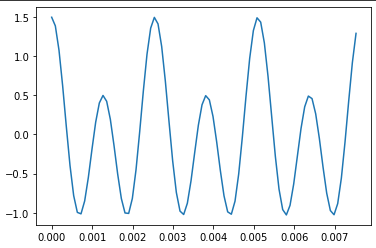
\includegraphics[scale=1]{fig/lab01/lab1_8.png}
		\caption{Суммированные сигналы}
	\end{center}
\end{figure}

\begin{lstlisting}[language=Python]
spectrum = wave.make_spectrum()
spectrum.plot(high = 1000)
\end{lstlisting}

\begin{figure}[H]
	\begin{center}
		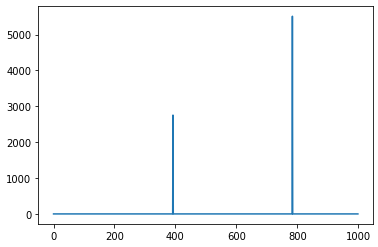
\includegraphics[scale=1]{fig/lab01/lab1_9.png}
		\caption{Спектр сигнала}
	\end{center}
\end{figure}

Добавим частоту из другой октавы. Должно получится ужасно для ушей.

\begin{lstlisting}[language=Python]
cos_signal3 = CosSignal(freq = 500, amp=0.25,offset = 0)
mix = mix + cos_signal3
wave = mix.make_wave(duration=1)
wave.make_audio()
\end{lstlisting}

На графике за 7мс не видно цикла.
\begin{figure}[H]
	\begin{center}
		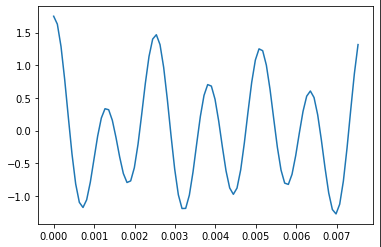
\includegraphics[scale=1]{fig/lab01/lab1_10.png}
		\caption{Получившийся сигнал}
	\end{center}
\end{figure}

Полученный звук не очень приятный.


\subsection{Упражнение 3}

Напишите функцию strech, берущую wave и коэффицент изменения. Она должна ускорять или замедлять сигнал изменением ts и framerate.

\noindent ts - моменты выборки сигнала, framerate - число выборок в единицу времени

\noindent если умножим ts на k - интервалы между моментами увеличатся в k раз

\noindent если framerate поделим на k - будет меньшее число подвыборок

\begin{lstlisting}[language=Python]
def stretch(wave, k):
  wave.ts *= k
  wave.framerate /= k
  return wave 
\end{lstlisting}


\subsection{Вывод}
В ходе первой ЛР я познакомился с основными понятиями при работе со звуками и сигналами в частности. Библиотека thinkDSP дает огромный потенциал для взаимодействия со звуками.